\documentclass[preprint,12pt]{elsarticle}
\usepackage{amsmath}
\usepackage{amssymb}
\usepackage{booktabs}
\usepackage{float}
\usepackage{graphicx}
\usepackage{multirow}
\usepackage{url}
\usepackage[hidelinks]{hyperref}
\emergencystretch=3em

\journal{Microelectronics Journal}
\biboptions{numbers,sort&compress}

\begin{document}

\begin{frontmatter}

\title{A Validation-Blind Simulator-in-the-Loop Stopping Protocol for Standard-Cell Delay Calibration Across Two Open PDKs}

\author[aff1]{Jiaqing Chen\corref{cor1}}
\ead{Jq\_Chen0715@buaa.edu.cn}

\author[aff1]{Feng Shao}
\cortext[cor1]{Corresponding author.}

\affiliation[aff1]{
organization={School of Integrated Circuit Science and Engineering, Beihang University},
addressline={No. 37 Xueyuan Road, Haidian District},
city={Beijing},
postcode={100191},
country={China}}

\begin{abstract}
Knowing when to stop a simulator-in-the-loop calibration is different from showing that a regressor fits a completed table. We present a validation-blind stopping protocol for pre-layout standard-cell delay calibration and test its evidence chain across GF180MCU and SKY130. A variant-balanced space-filling policy queries 16 released combinational-cell variants at an unseen process corner. Three deployment-observable signals---prequential error, prediction change, and feature-space coverage---must satisfy thresholds fixed on nine GF180MCU development pools for two consecutive batches. Estimator randomness is held constant across budgets. In completed-pool confirmation, the unchanged rule remains within 0.02 pooled delay $R^2$ of a measured 96-call reference in 5/6 GF180MCU pools and 15/15 SKY130 pools; among pools that actually stop before 96 calls, the corresponding counts are 2/3 and 8/8. We then run six new seed-5 pools prospectively: a hashed decision record and 80-call measurement snapshot are written before reference completion. Four pools stop at 80 calls, two fall back to 96, and all six satisfy the 0.02 criterion (maximum gap 0.0190). Fixed 48- and 64-call budgets are less reliable. Pooled ranking is stable, but per-variant audits expose negative $R^2$ for narrow-range cases, precluding a uniform cell-level accuracy claim. The 10,669-call evidence package therefore supports an auditable stopping method with PDK-specific retraining, not a new acquisition theory, zero-shot technology transfer, complete Liberty characterization, or sign-off.
\end{abstract}

\begin{keyword}
standard cells \sep GF180MCU \sep SKY130 \sep SPICE simulation \sep validation-blind stopping \sep sequential experimental design \sep process-corner calibration
\end{keyword}

\end{frontmatter}

\section{Introduction}

Transistor-level simulation remains the reference for evaluating standard-cell delay and power because these quantities depend jointly on transistor sizing, topology, process corner, voltage, temperature, load capacitance, and input transition time. Even before complete library characterization, a designer may need to explore many combinations to decide which regions deserve a denser sweep. The practical question is therefore not only whether a regression model fits previously generated rows, but whether it can allocate a limited budget of new SPICE simulations without hiding extrapolation failures.

Learning-assisted circuit design has been studied in analog, mixed-signal, and standard-cell settings \cite{Fayazi_AI_AMS_Review_2021,Afacan_ML_AnalogRF_Review_2021,Mina_ML_AnalogIC_Review_2022,Klemme_CellLib_ML_DTCO_ICCAD_2020,Klemme_Reliability_CellLib_TCASI_2021}. Bayesian and multi-fidelity methods have further shown that a simulator budget can be treated as part of the optimization problem rather than as a fixed data-collection cost \cite{Lyu_Bayesian_Analog_2018,Zhang_MultiFidelity_BO_DAC_2019,He_Batched_MultiFidelity_BO_TCAD_2023}. However, three gaps remain important for a small open-PDK study. First, a random split of a static table mainly measures interpolation. Second, pool-based replay does not prove that selected points were actually simulated during acquisition. Third, PDK control parameters can silently change the statistical meaning of the generated data.

The third issue is concrete in the GF180MCU flow used here. The included design configuration enables global and mismatch statistical switches by default. If these switches are not overridden, two nominally identical netlists can produce different values while the resulting table is described as a deterministic PVT study. That behavior may be appropriate for variation analysis, but it confounds a corner-calibration experiment unless random draws and seeds are modeled explicitly. We therefore force both switches off and retain the configuration, model path, netlist, and simulator log for every row.

This paper reframes the study around a simulator-in-the-loop methods question: a process corner is absent from the base training set; acquisition sees only the features of 96 new candidates; selected points are submitted to ngspice; and an independent validation set is excluded from selection and stopping. Completing the same pool later provides a measured reference. Released GF180MCU and SKY130 cells test whether a locked stopping procedure survives changes in device models and cell implementation, while a separate prospective stage records the stop decision before post-decision reference calls begin. The one-sentence claim is deliberately narrow: across two open-PDK combinational-cell studies, a deterministic, validation-blind sequential protocol can avoid some measured support calls while bounding pooled validation loss relative to completed candidate pools, with PDK-specific retraining and without a uniform per-variant guarantee. This design supports four contributions:

\begin{enumerate}
\item a deterministic GF180MCU/ngspice generation protocol that makes statistical-mode control, model corners, estimator randomness, netlists, and logs explicit and auditable;
\item a validation-blind unseen-corner support loop with fresh SPICE calls and matched acquisition baselines, establishing why a fixed budget learned from four controlled templates is not sufficient evidence for released cells;
\item a three-signal stopping rule developed on nine released-cell GF180MCU pools, locked before six same-PDK confirmation pools and 15 SKY130 protocol-replication pools, with conditional early-stop outcomes reported separately from 96-call fallbacks; and
\item a prospective six-pool confirmation in which hashed 80-call decision snapshots precede reference completion, together with exact descriptive intervals, signal ablations, cost accounting, ranking metrics, and worst-variant/tail-error audits.
\end{enumerate}

The method is deliberately bounded. It targets early transistor-level exploration of controlled and released combinational-cell arcs. Cross-PDK validation means replication of a fixed allocation and stopping protocol with PDK-specific training data; it does not mean direct transfer of one fitted regression model between technologies. The method does not replace sign-off simulation, layout-parasitic extraction, all timing arcs, leakage-state characterization, or complete Liberty generation.

\section{Related work and study position}

Machine-learning surrogates are widely used for expensive circuit-response prediction and design-space search \cite{Fayazi_AI_AMS_Review_2021,Afacan_ML_AnalogRF_Review_2021,Mina_ML_AnalogIC_Review_2022}. In standard-cell characterization, prior work has addressed library modeling, design-technology co-optimization, reliability, knowledge transfer, and graph representations \cite{Klemme_CellLib_ML_DTCO_ICCAD_2020,Klemme_Reliability_CellLib_TCASI_2021,Tang_KnowledgeTransfer_CellLib_MEJO_2025,Ma_GNN_CellLib_Integration_2025}. Those studies motivate learning-assisted characterization and provide model classes more sophisticated than the Extra Trees regressor used here. Our complementary focus is not a larger model zoo: it is the experimental protocol needed to demonstrate that a surrogate actually reduces fresh SPICE work, that stopping does not consult validation labels, and that failures remain visible after aggregation.

Sequential design and active learning choose the next expensive label using the current model or the geometry of the unlabeled pool \cite{Settles_ActiveLearning_2009}. In circuit optimization, Bayesian and multi-fidelity methods commonly combine prediction uncertainty, expected improvement, or fidelity-aware cost \cite{Lyu_Bayesian_Analog_2018,Zhang_MultiFidelity_BO_DAC_2019,He_Batched_MultiFidelity_BO_TCAD_2023}. Our purpose is narrower. We do not claim a new acquisition theory. We test whether a simple policy can be executed as an auditable SPICE loop and how much measured work it saves relative to completing the same candidate pool.

This distinction matters for journal positioning. Model-zoo results are retained only as a same-flow sanity check. The main unit of evidence is a SPICE query, not a row revealed retrospectively from a labeled table. The main comparison is against a measured exhaustive candidate set, not only against another regressor on a random split. Table~\ref{tab:study-position} makes the claim boundary explicit.

\begin{table}[t]
\centering
\caption{Position of the present methods-validation study relative to adjacent work.}
\label{tab:study-position}
\small
\setlength{\tabcolsep}{4pt}
\begin{tabular}{p{0.16\textwidth}p{0.17\textwidth}p{0.24\textwidth}p{0.30\textwidth}}
\toprule
Study class & Main evidence unit & Typical primary question & Present distinction \\
\midrule
Cell-library ML \cite{Klemme_CellLib_ML_DTCO_ICCAD_2020,Klemme_Reliability_CellLib_TCASI_2021,Tang_KnowledgeTransfer_CellLib_MEJO_2025,Ma_GNN_CellLib_Integration_2025} & Prediction set & Can cell responses be modeled efficiently? & Not an acquisition or stopping audit \\
Bayesian and multi-fidelity search \cite{Lyu_Bayesian_Analog_2018,Zhang_MultiFidelity_BO_DAC_2019,He_Batched_MultiFidelity_BO_TCAD_2023} & Sequential expensive evaluation & Which design should be evaluated next? & Optimization-centered rather than cross-PDK stop confirmation \\
This work & Measured SPICE call and decision artifact & When can unseen-corner support stop without validation labels? & Locked rule, completed references, prospective decision-before-completion test \\
\bottomrule
\end{tabular}
\end{table}

\section{Deterministic SPICE protocol}

\subsection{PDK, simulator, and statistical-mode control}

All publication-eligible simulations use ngspice 46 \cite{Ngspice_Manual}. The GF180MCU stages use the primitive-device model file \texttt{sm141064.ngspice} \cite{Google_GF180MCU_PDK_GitHub,GF180MCU_ReadTheDocs_CustomDesign,GF180MCU_Model_sm141064}. The local PDK checkout corresponds to commit \texttt{de3240d}; the primitive-model and 7-track standard-cell submodules correspond to commits \texttt{9f992d5} and \texttt{43beb45}, respectively \cite{GF180MCU_ReadTheDocs_StdCells_7Track}. The full hashes are given in the repository references. The controlled templates use \texttt{nmos\_3p3} and \texttt{pmos\_3p3}. The released-cell experiment instantiates official cell CDLs and preserves their transistor connectivity, widths, and lengths while mapping their 5-V device symbols to compatible open ngspice model wrappers.

The cross-PDK stage uses the FOSSi Foundation SKY130 primitive-device and high-density standard-cell repositories at commits \texttt{403964d} and \texttt{9cb2d7c}, respectively \cite{FOSSi_SKY130_Primitive_GitHub,FOSSi_SKY130_HD_GitHub}. Generated standard-cell SPICE subcircuits instantiate \texttt{sky130\_fd\_pr\_\_nfet\_01v8} and \texttt{sky130\_fd\_pr\_\_pfet\_01v8\_hvt}. Each netlist includes only the corresponding official tt, ff, or ss PM3 models and their mismatch-parameter definitions. The mismatch and process-randomization switches \texttt{mc\_mm\_switch} and \texttt{mc\_pr\_switch} are set to zero, so this stage has the same deterministic estimand as the GF180MCU study.

The GF180MCU design include enables both global and mismatch statistical switches by default. Each generated publication netlist therefore inserts

\begin{verbatim}
.param sw_stat_global=0 sw_stat_mismatch=0
\end{verbatim}

after the design include. This override defines the reported experiment as deterministic corner characterization rather than Monte Carlo variation analysis. The dataset records \texttt{statistical\_mode=off}, both switch values, the sampling seed, simulator version, model path, netlist path, log path, fidelity, and completion status.

Threshold voltage is not entered as a free scalar regressor feature. It is embedded in the PDK device equations and selected implicitly when the netlist includes the tt, ff, or ss model section; the corresponding categorical corner is provided to the surrogate. This choice preserves each PDK's internally consistent mobility, threshold, capacitance, and temperature dependencies instead of treating $V_{\mathrm{th}}$ as an independently adjustable number. It also explains why model parameters are not transferred between PDKs: each technology is retrained on its own measured rows.

\subsection{Cells, variables, and measured targets}

The templates cover controlled arcs for INV, NAND2, NOR2, and XOR2. NAND2 and NOR2 use tied-input transitions. XOR2 holds one input high while the other toggles. The experiment therefore studies controlled topology cases rather than every legal state and timing arc of a production cell library.

The numerical inputs are NMOS width $W_n$, channel length $L$, PMOS/NMOS width ratio, supply voltage, temperature, load capacitance, and input slew. Cell type, input arc, and process corner are categorical inputs. The channel length is fixed at 0.28~$\mu$m. The targets are average propagation delay,
\begin{equation}
d=\frac{t_{\mathrm{PHL}}+t_{\mathrm{PLH}}}{2},
\end{equation}
and average switching supply power over the defined transient measurement window. Numerical features are standardized and categorical features are one-hot encoded with unknown-category-safe handling. The controlled experiment assigns each simulated point one of four non-overlapping data roles. Table~\ref{tab:protocol} lists their sizes, label-access rules, sampling functions, and retained provenance.

\begin{table}[H]
\centering
\caption{Controlled-stage deterministic datasets and simulator-in-the-loop protocol.}
\label{tab:protocol}
\resizebox{\textwidth}{!}{%
\begin{tabular}{lllll}
\toprule
Component & Size & Sampling role & Label access & Provenance \\
\midrule
Primary SPICE set & 320 rows; 80/cell & Base training and development & Available before online study & Netlist, log, model, switches \\
Validation SPICE set & 480 rows; 120/cell & Independent budget evaluation & Never available to acquisition & Separate sampling seed/directories \\
Online candidate pool & 96 points per seed-corner & Same-corner support search & Features only until selected & Fresh netlist and log per query \\
Measured reference & 96 points per seed-corner & Exhaustive budget reference & Completed after online runs & One retained row per candidate \\
\midrule
Seeds and corners & \multicolumn{4}{l}{Five pool seeds; held-out ff, ss, and typical corners; four-query batches; maximum online budget 48} \\
Variable ranges & \multicolumn{4}{l}{$W_n$: 0.517--4.990~$\mu$m; ratio: 1.503--2.999; $V_{DD}$: 1.620--1.980~V; temperature: $-20$--100~$^\circ$C; load: 1.066--99.832~fF; slew: 10.672--499.454~ps} \\
\bottomrule
\end{tabular}}
\end{table}

\subsection{Independent datasets}

The primary dataset contains 320 successful rows generated with Latin hypercube seed 20260530. Each cell contributes 80 rows. The corner counts are 104 ff, 108 ss, and 108 typical rows. The independent validation dataset contains 480 successful rows generated with seed 20260602, with 120 rows per cell and 160 rows per corner. No legacy or externally sourced table is included in the reported training, support, or evaluation sets.

The independent validation set is not cross-PDK or cross-simulator validation. Both datasets use the same PDK, simulator, device models, and circuit templates. Independence here means a different design-point sample, sampling seed, netlist directory, and log directory within the same controlled flow.

\section{Released-library and cross-PDK external validation}

\subsection{Official CDLs and independent datasets}

To test whether conclusions from author-defined templates survive a more realistic topology distribution, we construct a second experiment from the released GF180MCU 7-track standard-cell CDLs. The set contains INV, NAND2, NOR2, XOR2, AOI21, OAI21, MUX2, and NAND3 families at drive strengths 1 and 4, giving 16 cell variants. One sensitized input arc is used per family. For the ngspice flow, official CDL instances of \texttt{nfet\_05v0} and \texttt{pfet\_05v0} are mapped to the open \texttt{nmos\_6p0} and \texttt{pmos\_6p0} subcircuit wrappers while preserving transistor connectivity, width, and length. This is a released-topology external test within the same PDK, not a claim of bit-identical reproduction of the library provider's characterization deck.

Independent primary and validation datasets contain 576 successful rows each, generated with seeds 20260717 and 20260731. Each dataset contains 36 points per variant and 192 points per process corner. Besides voltage, temperature, input slew, load, and corner, the model receives family, variant, drive strength, sensitized arc, input count, transistor count, and aggregate NMOS/PMOS width. The joint sampled range is 1.62--1.98~V, $-40$--125~$^\circ$C, 0.02--12~ns input slew, and 0.001--0.206~pF load.

The online study uses five additional pool seeds and three held-out corners. Each pool contains six unseen points for every variant, or 96 candidates. A variant-balanced farthest-first order is generated from feature geometry, and support is added in 16-query batches so that every variant receives one point per batch. Completing all 15 pools requires 1440 fresh, successful SPICE calls and supplies the measured references used below.

\subsection{Validation-blind stopping rule}

The released-library stages use an Extra Trees delay regressor with 320 trees, \texttt{min\_samples\_leaf=2}, all transformed features available at each split, and a random state fixed to the pool seed at every budget. Consequently, prediction change reflects added SPICE support rather than a different ensemble realization. Numerical inputs are standardized; family, variant, sensitized arc, and corner are one-hot encoded with unknown categories ignored. The implementation uses Python 3.10, scikit-learn 1.7.2, pandas 2.3.3, NumPy 2.2.6, and SciPy 1.15.3.

Let $D_{k-1}$ be the available training data before batch $B_k$, $f_k$ the model after adding that batch, $P$ the feature-only 96-point pool, and $S_k$ the selected candidates. Normalization uses
\begin{equation}
s(D)=\max\{\operatorname{IQR}(y_D),\,0.1\operatorname{median}(|y_D|),\,10^{-12}\}.
\end{equation}
The three deployment-observable signals are prequential error,
\begin{equation}
E_k=\frac{\operatorname{MAE}(y_{B_k},f_{k-1}(B_k))}{s(D_{k-1})},
\end{equation}
prediction change over the full feature pool,
\begin{equation}
P_k=\frac{\operatorname{median}_{x\in P}|f_k(x)-f_{k-1}(x)|}{s(D_k)},
\end{equation}
and coverage radius,
\begin{equation}
C_k=\frac{\max_{x\in P\setminus S_k}\min_{z\in S_k}\lVert g(x)-g(z)\rVert_2}{C_0},
\end{equation}
where $g$ standardizes voltage, temperature, slew, and load and $C_0$ is the initial centroid-based radius. No independent-validation label appears in these quantities. Seeds 0--2 (nine corner pools) select thresholds from a 400-rule grid. A candidate must keep at least eight of nine development runs within 0.02 pooled delay $R^2$ of the full reference and every development run within 0.05. The selected rule requires a minimum budget of 64, $E_k\leq0.25$, $P_k\leq0.05$, and $C_k\leq0.50$ for two consecutive batches. These values are locked before seeds 3--4 (six same-PDK confirmation pools) and every SKY130 pool are evaluated.

\subsection{SKY130 external protocol replication}

The locked rule is next applied to a second open PDK without threshold selection or retuning. The SKY130 high-density set contains the same eight logical families and drive strengths 1 and 4. SKY130 names AOI21 and OAI21 as \texttt{a21oi} and \texttt{o21ai}; the analysis retains the common logical-family names while recording every original source-cell name and path. One sensitized arc is selected per family using the same logical conditions as in the GF180MCU released-cell study.

Independent SKY130 primary and validation datasets contain 576 successful rows each, generated with seeds 20260718 and 20260819. Each dataset contributes 36 points per variant and 192 points per corner. The sampled voltage, temperature, slew, and load ranges are identical to the released GF180MCU study. Five new pool seeds and three held-out corners provide 15 additional 96-point pools. Acquisition uses the same variant-balanced farthest-first order and 16-query batches. For each corner, the regressor is trained on SKY130 data from the other two corners and updated with newly measured same-corner support. Thus, this experiment tests transfer of the allocation and stopping protocol, not transfer of fitted GF180MCU model parameters.

All 1440 candidate netlists are simulated to obtain measured 96-call references. The stopping decision is then replayed sequentially using the unchanged GF180MCU thresholds. This completed-pool analysis is useful for matched error measurement but, by itself, is not evidence that a decision preceded the unqueried calls. We therefore label the 15 SKY130 and six GF180MCU locked cohorts as completed-pool confirmation rather than prospective stopping. The two independent SKY130 datasets and online pools add 2592 successful calls. Netlists, logs, source-cell paths, PDK commits, model corners, and switch values are retained for audit.

\subsection{Prospective decision-before-completion confirmation}

After the thresholds, acquisition order, batch size, estimator random-state policy, and analysis code are frozen, seed 5 supplies one new pool per corner and PDK, or six prospective pools. Before the first call in each pool, a precommit manifest records the rule and SHA-256 hashes of the relevant source and primary-training data; it declares but does not open the validation path. Simulations then run in 16-query batches. When two consecutive batches are eligible, the program writes a decision record and a hashed measurement snapshot before launching any remaining calls. If the rule is not triggered, the pool records a full-budget fallback at 96. Only after this artifact exists are the independent validation labels opened and the remaining candidates, if any, used to construct the measured reference. These 576 new calls increase the complete evidence package from 10,093 to 10,669 successful simulations.

\subsection{Partial Liberty compatibility check}

As a separate engineering check, released Liberty delay surfaces are compared with fresh simulations of the corresponding released CDLs. For each of 16 variants and three matched PVT files, the low, middle, and high indices of both the ten-point slew axis and ten-point load axis form nine comparison points, giving 432 simulations. We report rank and absolute agreement separately. This experiment is intentionally partial: it does not reconstruct all arcs, constraints, leakage states, internal power groups, waveform settings, or extracted parasitics of a complete characterization flow.

\section{Simulator-in-the-loop corner calibration}

\subsection{Held-out-corner task}

For a held-out corner $c$, the base set contains only primary rows from the other two corners. A new candidate pool contains 24 Latin-hypercube points per controlled cell, or 96 points in total, all assigned to $c$. Acquisition initially receives only their input features. When a point is selected, the program writes its transistor-level netlist, launches ngspice, parses delay and power, appends the measured row to the support set, and retrains the surrogate. In the controlled and completed-pool studies, validation rows from corner $c$ record the budget trajectory but are not passed to acquisition or stopping logic. In the prospective study, the validation file remains unopened until a decision artifact exists. This information boundary is central to the simulation-saving claim. Fig.~\ref{fig:workflow} traces the original label flow and locked-rule sequence.

\begin{figure}[H]
\centering
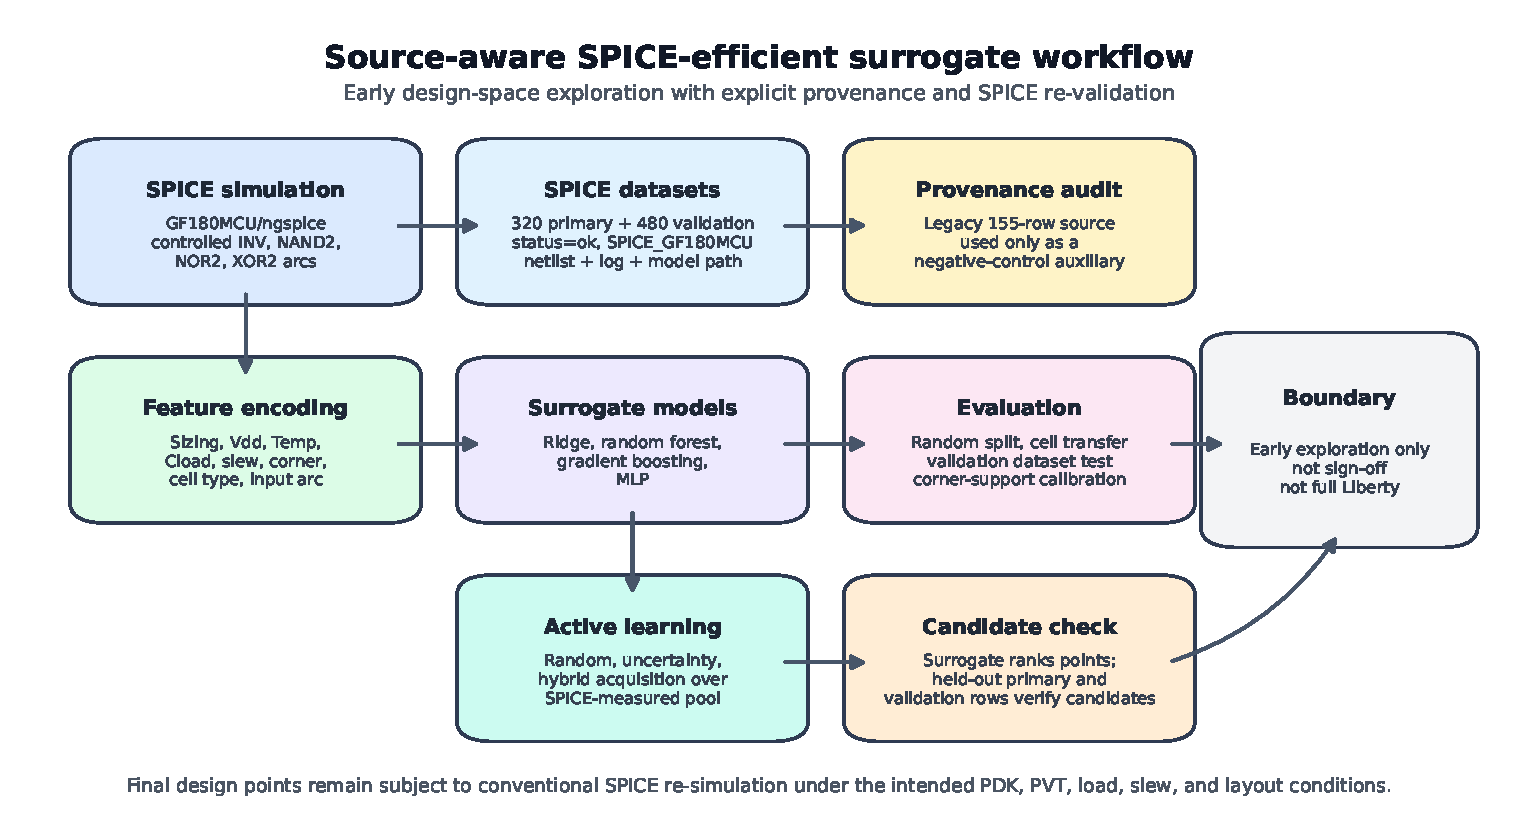
\includegraphics[width=\textwidth]{figures/fig1_workflow.pdf}
\caption{Validation-blind simulator-in-the-loop acquisition and locked-rule cross-PDK validation. \textbf{(a)} For a held-out corner, acquisition receives a feature-only 96-point pool. Every selected support label is obtained from a fresh ngspice run, whereas independent validation labels are excluded from selection and stopping; completing the pool provides the measured exhaustive reference. \textbf{(b)} Observable thresholds are selected on nine GF180MCU development pools, locked before six same-PDK confirmation pools and 15 SKY130 external pools are examined, and applied without retuning. A later six-pool prospective stage writes each decision before reference completion. Models are retrained within each PDK; the experiment is pre-layout and is not zero-shot parameter transfer or complete Liberty characterization.}
\label{fig:workflow}
\end{figure}

\subsection{Surrogate and acquisition strategies}

The online support model is an Extra Trees regressor with 240 trees, \texttt{min\_samples\_leaf=2}, and all transformed features available at each split. Separate models predict delay and power. This model is fixed across all strategies. Its purpose is to provide a stable nonlinear support model, not to establish a new model-ranking result.

For geometric selection, standardized numerical features are concatenated with one-hot cell indicators. Let $g(x)$ denote this vector and $S$ the queried set. The diversity score is
\begin{equation}
q_{\mathrm{div}}(x)=
\begin{cases}
\min_{s\in S}\lVert g(x)-g(s)\rVert_2, & S\neq\emptyset,\\
\lVert g(x)-\bar g\rVert_2, & S=\emptyset,
\end{cases}
\end{equation}
where $\bar g$ is the candidate-pool centroid. Each four-query cell-balanced space-filling batch selects one available point from each cell with the largest current diversity score. A primary-data-only development study fixed the policy to pure diversity before the independent online evaluation.

Five policies use identical pools: random selection, cell-balanced random selection, uncertainty-only selection from tree-ensemble disagreement, ordinary greedy space filling, and cell-balanced space filling. The last policy is the operational method studied here. It guarantees equal support counts across the four cells at every completed batch. We do not assume that it must outperform ordinary space filling; the comparison tests whether cell balance changes reliability or cost.

\subsection{Evaluation and statistics}

After budgets $b\in\{0,4,\ldots,48\}$, the model is evaluated on all 160 validation rows from the held-out corner. We report delay and power $R^2$, MAE, the minimum delay $R^2$ across the four cells, Spearman correlation, Kendall's tau, top-20\% precision and recall, and NDCG. The main metric is independent-validation delay $R^2$ because delay shows the strongest zero-shot corner failure.

The complete design has five seeds, three held-out corners, and five strategies, yielding 75 online runs and 3600 actual ngspice queries. Seventy-seven additional calls complete candidates not selected by any strategy. The online and completion phases therefore contain 3677 new simulator calls and 2311.5~s of measured serial-equivalent wall time.

At budgets 24 and 48, the cell-balanced space-filling policy is compared with each baseline over 15 matched seed-corner pairs using two-sided Wilcoxon signed-rank tests. Holm correction is applied within each budget-metric family. The paired design prevents differences among candidate-pool seeds or corners from being mistaken for acquisition effects.

For stopping studies, success is defined before confirmation as a pooled delay-$R^2$ gap no greater than 0.02 relative to the corresponding measured 96-call model. We report all-pool results, genuinely early-stopped pools ($b<96$), and full-budget fallbacks separately. Exact two-sided Clopper--Pearson 95\% intervals accompany success proportions. Because three corners share a PDK and sampling design, these intervals are descriptive finite-cohort summaries rather than proof of independent population coverage. Robustness outputs also include per-variant $R^2$, MAE, normalized MAE, 95th-percentile and maximum absolute error, pooled Spearman correlation, top-20\% slowest-cell recall, a 400-rule threshold grid, and removal of each stopping signal. Model fitting/prediction time is measured separately from the sum of per-call ngspice engine times.

\section{Results}

\subsection{Configuration control restores numerical repeatability}

The first result is methodological rather than predictive. Before the statistical-mode override, repeated nominal candidate simulations differed because global and mismatch variation were enabled by the included PDK configuration. With both switches forced to zero, independently launched repeats are identical. Across the online study, 1118 candidate groups were queried by at least two strategies, accounting for 3355 query records. The maximum within-group span is exactly 0 for $t_{\mathrm{PHL}}$, $t_{\mathrm{PLH}}$, average delay, and average power at the stored precision. This audit prevents stochastic PDK variation from being misreported as deterministic PVT response or acquisition noise.

As a secondary same-flow sanity check, models trained on all 320 primary rows generalize to the independently sampled 480-row validation set. CatBoost reaches delay $R^2=0.9208$ and MAE 0.0321~ns, while Gaussian-process regression reaches power $R^2=0.9994$ and MAE 0.0449~$\mu$W. These values show that the deterministic tables are learnable, but they are not the main evidence for simulation reduction.

\subsection{Same-corner queries repair delay extrapolation}

Without same-corner support, the cell-balanced space-filling trajectory has pooled median delay $R^2=0.4825$ over the 15 seed-corner pairs. The corner dependence is substantial: median zero-support $R^2$ is 0.3055 for ff, 0.4825 for ss, and 0.7877 for typical. This confirms that a strong random-split or same-flow validation score does not justify zero-shot use at an absent corner.

Fresh same-corner SPICE labels improve the difficult corners. At 24 queries, median delay $R^2$ reaches 0.7763 for ff, 0.8035 for ss, and 0.8896 for typical. At 48 queries, the values are 0.8797, 0.8488, and 0.8887. The pooled worst-cell delay $R^2$ rises from 0.3112 without support to 0.6785 at 24 queries and 0.7885 at 48 queries. Power changes little because its zero-support transfer is already strong: pooled median power $R^2$ is 0.9455 at zero support and 0.9465 at 48 queries. Table~\ref{tab:corner-results} resolves these trends by held-out corner and compares each support budget with its measured 96-query reference and simulation time.

\begin{table}[t]
\centering
\caption{Cell-balanced space-filling results by held-out corner. Values are medians over five candidate-pool seeds.}
\label{tab:corner-results}
\resizebox{\textwidth}{!}{%
\begin{tabular}{llrrrr}
\toprule
Corner & Support & Delay $R^2$ & Worst-cell delay $R^2$ & Top-20\% recall & Measured time (s) \\
\midrule
\multirow{4}{*}{ff} & 0 & 0.3055 & $-0.1887$ & 0.8750 & 0.00 \\
 & 24 & 0.7763 & 0.6000 & 0.8750 & 14.40 \\
 & 48 & 0.8797 & 0.7883 & 0.8750 & 28.88 \\
 & 96 reference & 0.9054 & 0.8539 & 0.8750 & 59.62 \\
\midrule
\multirow{4}{*}{ss} & 0 & 0.4825 & 0.3112 & 0.9688 & 0.00 \\
 & 24 & 0.8035 & 0.7060 & 0.9688 & 14.38 \\
 & 48 & 0.8488 & 0.7925 & 0.9688 & 28.86 \\
 & 96 reference & 0.8541 & 0.7853 & 0.9688 & 59.20 \\
\midrule
\multirow{4}{*}{typical} & 0 & 0.7877 & 0.4872 & 0.8125 & 0.00 \\
 & 24 & 0.8896 & 0.7755 & 0.8750 & 14.40 \\
 & 48 & 0.8887 & 0.7983 & 0.9062 & 28.87 \\
 & 96 reference & 0.8824 & 0.7918 & 0.9375 & 58.73 \\
\bottomrule
\end{tabular}}
\end{table}

\subsection{Space coverage is safer than uncertainty-only acquisition}

To separate acquisition-policy effects from the benefit of support volume alone, Fig.~\ref{fig:online-results}(a--c) compares matched budget trajectories. At 24 queries, cell-balanced space filling has pooled median delay $R^2=0.8119$, compared with 0.7625 for random, 0.7812 for cell-balanced random, 0.8114 for ordinary space filling, and 0.7232 for uncertainty-only selection. The difference from uncertainty-only selection remains significant after Holm correction ($p=0.0171$). The difference from random is positive but does not cross the corrected 0.05 threshold ($p=0.0646$).

At 48 queries, the respective medians are 0.8729, 0.8564, 0.8685, 0.8674, and 0.8111. Cell-balanced space filling exceeds random ($p=0.0374$) and uncertainty-only selection ($p=0.0334$) after correction. It is statistically indistinguishable from cell-balanced random and ordinary space filling ($p=1.0$ for both corrected comparisons). The worst-cell advantage over random is not significant after correction ($p=0.1414$). These tests support a restrained conclusion: covering the new corner is safer than relying only on ensemble disagreement, while the present data do not demonstrate superiority over all space-filling alternatives.

Cell balance is nevertheless operationally explicit. Its support-count range is zero at every complete four-query batch. At 48 queries, the median range is four points for random, ordinary space filling, and uncertainty-only selection. This property prevents one cell from consuming most of a small support budget even when aggregate accuracy appears acceptable. Fig.~\ref{fig:online-results}(d) then places the selected 24- and 48-query budgets against the distribution of measured 96-query references.

\begin{figure}[H]
\centering
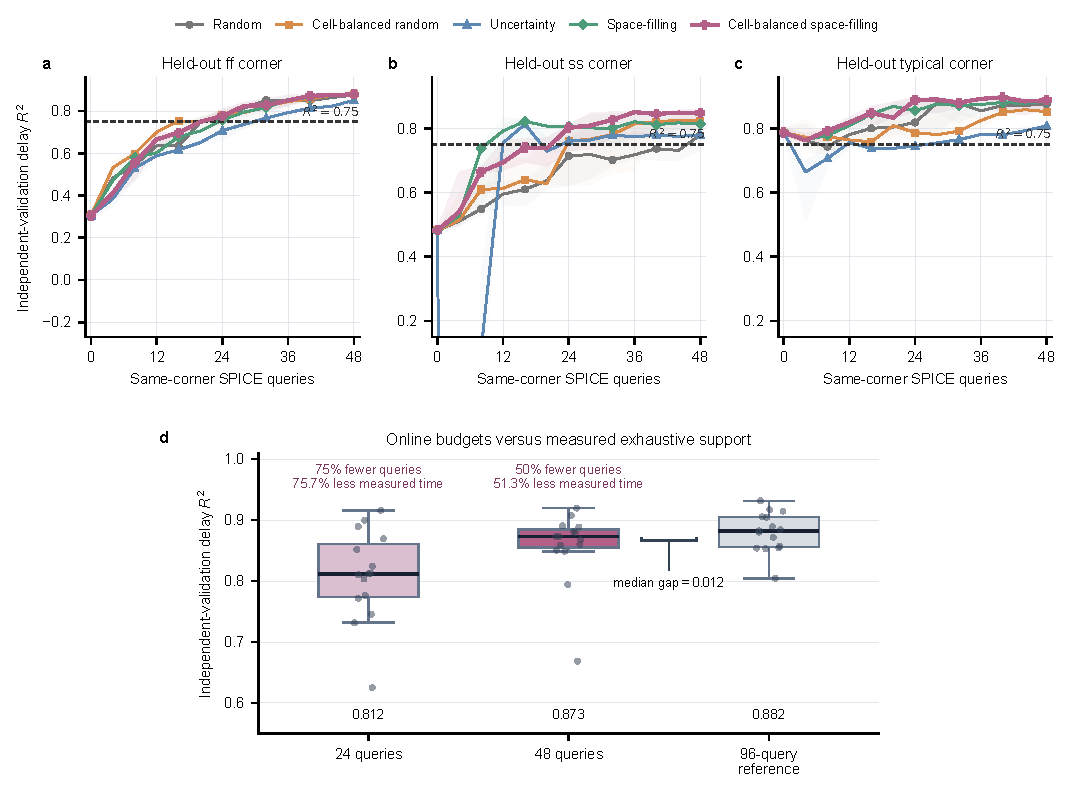
\includegraphics[width=\textwidth]{figures/fig2_online_corner_calibration.pdf}
\caption{Validation-blind simulator-in-the-loop results. (a--c) Median independent-validation delay $R^2$ across five seeds for each held-out process corner; translucent bands show the interquartile range. The horizontal line is the prespecified $R^2=0.75$ study threshold. (d) Distribution over 15 matched seed-corner runs for cell-balanced space filling at 24 and 48 queries and for the measured 96-query reference. Each point is one seed-corner pair. The 48-query budget reduces SPICE calls by 50\% and measured time by 51.3\%, with a median $R^2$ gap of 0.012 to the full reference.}
\label{fig:online-results}
\end{figure}

\subsection{Half of the measured candidate pool approaches the exhaustive reference}

Completing every candidate produces 15 measured 96-query references, one for each seed-corner pool. Their pooled median delay $R^2$ is 0.8824, median worst-cell delay $R^2$ is 0.8150, and median top-20\% recall is 0.9375. With 24 queries, cell-balanced space filling uses 75\% fewer calls and 75.7\% less measured time; median delay $R^2$ is 0.8119 and the median gap to the reference is 0.0798. With 48 queries, call reduction is 50\%, time reduction is 51.3\%, median delay $R^2$ is 0.8729, and the median gap is 0.0120.

The 48-query budget also preserves the reference median top-20\% recall of 0.9375. Its median worst-cell delay $R^2$ is 0.7885, compared with 0.8150 for the reference. These results quantify the engineering trade-off directly: half of the candidate simulations retain most of the measured support benefit, whereas one quarter of the pool is useful but leaves a larger accuracy gap. Table~\ref{tab:exhaustive} consolidates the resulting call, time, accuracy, and ranking-recall trade-offs.

\begin{table}[t]
\centering
\caption{Online budgets compared with the measured 96-query reference over 15 seed-corner runs.}
\label{tab:exhaustive}
\resizebox{\textwidth}{!}{%
\begin{tabular}{lrrrrrr}
\toprule
Support & Query reduction & Time reduction & Delay $R^2$ & Gap to reference & Worst-cell $R^2$ & Top-20\% recall \\
\midrule
24 queries & 75.0\% & 75.7\% & 0.8119 & 0.0798 & 0.6785 & 0.8750 \\
48 queries & 50.0\% & 51.3\% & 0.8729 & 0.0120 & 0.7885 & 0.9375 \\
96-query reference & 0 & 0 & 0.8824 & 0 & 0.8150 & 0.9375 \\
\bottomrule
\end{tabular}}
\end{table}

\subsection{Validation-blind prequential error is informative but not a stopping guarantee}

For each four-query batch, predictions are recorded before its SPICE labels are added. This prequential error is observable during operation and does not use the independent validation labels. Across 180 batches, prequential delay MAE correlates negatively with external delay $R^2$ (Spearman $\rho=-0.3869$, $p=8.09\times10^{-8}$) and external worst-cell delay $R^2$ ($\rho=-0.3352$, $p=4.22\times10^{-6}$). The direction is useful, but the magnitude is only moderate. We therefore treat prequential error as a diagnostic for suspicious batches, not as a validated automatic stopping rule.

\subsection{The protocol transfers to released standard-cell CDLs}

All 1152 independently generated released-CDL rows and all 1440 online candidate simulations complete successfully with the statistical switches disabled. The released-library task is materially harder than the controlled four-topology stage. With estimator randomness fixed across budgets, median delay $R^2$ over 15 seed-corner pools is 0.2171 without target-corner support, 0.8217 at 32 queries, 0.8633 at 48, 0.8967 at 80, and 0.9097 after all 96 candidates are measured. Median worst-family $R^2$ rises from $-0.1009$ at zero support to 0.3722 at 48 and 0.7196 at 96. Table~\ref{tab:released-budgets} reports the pooled budget trade-off, while Fig.~\ref{fig:released-validation}(a) resolves the trajectory by held-out corner.

\begin{table}[t]
\centering
\caption{Released-CDL external-validation budgets over 15 seed-corner pools. Values are pooled medians.}
\label{tab:released-budgets}
\resizebox{\textwidth}{!}{%
\begin{tabular}{rrrrr}
\toprule
Support & Delay $R^2$ & Gap to reference & Worst-family $R^2$ & Measured time (s) \\
\midrule
0 & 0.2171 & 0.6863 & $-0.1009$ & 0.00 \\
32 & 0.8217 & 0.0975 & 0.1484 & 61.09 \\
48 & 0.8633 & 0.0525 & 0.3722 & 92.58 \\
80 & 0.8967 & 0.0134 & 0.6409 & 157.25 \\
96 reference & 0.9097 & 0 & 0.7196 & 185.60 \\
\bottomrule
\end{tabular}}
\end{table}

This transfer test changes the interpretation of the controlled result. A fixed 48-query budget is within 0.02 of the reference in only one of six untouched confirmation pools; its median gap is 0.0392 and maximum gap is 0.1424. The validation-blind rule instead stops at a median of 88 queries. Five of six confirmation runs are within 0.02, all six are within 0.05, and the maximum gap is 0.0226. The corresponding median delay $R^2$ is 0.9038 and median worst-family $R^2$ is 0.7389. Fig.~\ref{fig:released-validation}(b) shows that the rule is conservative, with a median query reduction of only 8.3\%. The all-pool success proportion is 5/6 (exact descriptive 95\% interval 0.359--0.996), but only three pools actually stop at 80; two of those three meet the 0.02 limit. The other three successes are full-budget fallbacks and must not be interpreted as saved simulations.

Fig.~\ref{fig:released-validation}(c) tests a different question: whether fresh ngspice simulations preserve the ordering and magnitude of released Liberty delays. Spearman $\rho=0.9900$, Pearson $r=0.9916$, and $R^2=0.9460$ indicate strong agreement in ordering and linear association. However, the median absolute percentage error is 18.58\%, and the median SPICE-to-Liberty delay ratio is 0.814. The ordering agreement supports early ranking, whereas the absolute bias confirms that the present deck does not replace the provider's complete characterization conditions.

\begin{figure}[t]
\centering
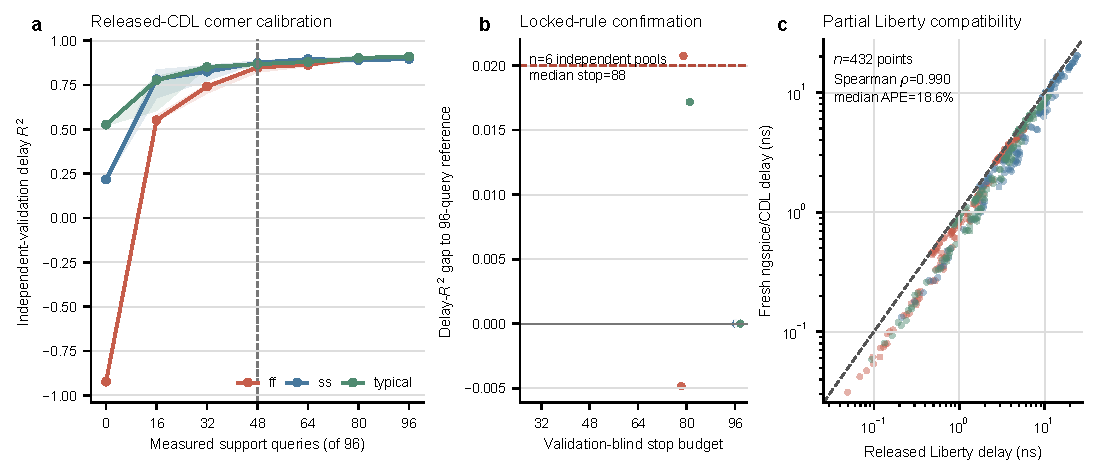
\includegraphics[width=\textwidth]{figures/fig3_official_library_validation.pdf}
\caption{External validation on released GF180MCU standard-cell CDLs. (a) Median independent-validation delay $R^2$ versus measured support for the three held-out corners; bands show the interquartile range over five pool seeds. (b) Untouched confirmation pools compare the validation-blind stopping budget with the resulting gap to each measured 96-query reference. Dashed lines mark gaps of 0.02 and 0.05. (c) Fresh ngspice delay versus official Liberty delay at 432 matched cell--PVT--slew--load points. The log--log identity line exposes the absolute offset while rank correlation quantifies ordering agreement.}
\label{fig:released-validation}
\end{figure}

\subsection{The GF180MCU stopping rule transfers to SKY130 without retuning}

The decisive transfer question is whether the GF180MCU-locked rule controls error better than fixed budgets on SKY130. Table~\ref{tab:cross-pdk-stopping} summarizes this matched comparison across both PDKs. The prelocked rule satisfies the primary 0.02-gap criterion in all 15 SKY130 completed pools (exact descriptive 95\% interval 0.782--1.000). Its median stop is 80 of 96 calls, corresponding to a 16.7\% median reduction, and its largest delay $R^2$ gap to a measured reference is 0.0110. The median stopped-model delay $R^2$ is 0.9032, and the median worst-family $R^2$ is 0.7004. Eight pools actually stop at 80 and all eight meet the limit (interval 0.631--1.000); seven, including all five ss pools, continue to 96 and therefore save no calls.

Fixed budgets do not provide the same protection. A 64-call budget meets the 0.02 criterion in 5 of 15 SKY130 pools and produces a maximum gap of 0.0943. A 48-call budget meets it in 2 of 15 pools and produces a maximum gap of 0.1491. The same ordering is present in the six untouched GF180MCU confirmation pools: the locked rule succeeds in five, whereas each fixed budget succeeds in one. To determine whether the aggregate rates hide corner-specific failures, Fig.~\ref{fig:cross-pdk} shows every locked-rule outcome and the matched fixed-budget comparisons. The result supports replication of the stopping protocol across these two PDKs, but it does not imply that a regressor fitted on GF180MCU directly predicts SKY130 cells.

\begin{table}[H]
\centering
\caption{Stopping-rule replication across released GF180MCU and SKY130 standard cells. Success means a delay $R^2$ gap no greater than 0.02 relative to the measured 96-call reference.}
\label{tab:cross-pdk-stopping}
\resizebox{\textwidth}{!}{%
\begin{tabular}{llrrrrr}
\toprule
PDK & Method & Pools & Median calls & Median reduction & Successful pools & Maximum gap \\
\midrule
GF180MCU & Locked rule & 6 & 88 & 8.3\% & 5/6 & 0.0226 \\
GF180MCU & Fixed 64 & 6 & 64 & 33.3\% & 1/6 & 0.0580 \\
GF180MCU & Fixed 48 & 6 & 48 & 50.0\% & 1/6 & 0.1424 \\
SKY130 & GF180MCU-locked rule & 15 & 80 & 16.7\% & 15/15 & 0.0110 \\
SKY130 & Fixed 64 & 15 & 64 & 33.3\% & 5/15 & 0.0943 \\
SKY130 & Fixed 48 & 15 & 48 & 50.0\% & 2/15 & 0.1491 \\
\bottomrule
\end{tabular}}
\end{table}

\begin{figure}[H]
\centering
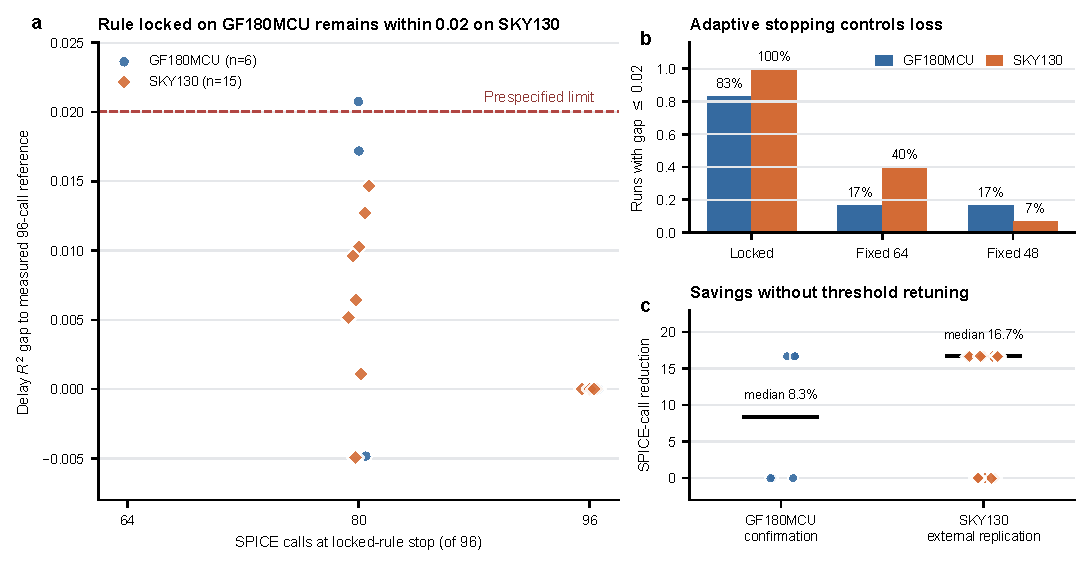
\includegraphics[width=\textwidth]{figures/fig4_cross_pdk_replication.pdf}
\caption{Cross-PDK replication of the validation-blind stopping rule. (a) Individual outcomes for the six untouched GF180MCU confirmation pools and 15 external SKY130 pools. The rule was selected using separate GF180MCU development pools; the dashed line is the prespecified 0.02 delay-$R^2$ gap limit. Negative gaps indicate that an early model slightly outperformed the corresponding 96-call model on the independent validation set. (b) Fraction of pools within the 0.02 limit for the locked rule and fixed 64- and 48-call budgets. (c) Call reduction for each locked-rule outcome; horizontal bars show medians. SKY130 thresholds were not retuned, and all candidate pools were completed to obtain measured references.}
\label{fig:cross-pdk}
\end{figure}

\subsection{Prospective confirmation separates decisions from reference completion}

The six seed-5 pools provide the chronological test that completed-pool replay cannot. Table~\ref{tab:prospective} summarizes the results. Typical and ff pools stop at 80 for both PDKs; both ss pools fall back to 96 because the two-consecutive-batch condition is not met. All six decisions are within 0.02 pooled delay $R^2$ of the subsequently completed references. The combined proportion is 6/6 (exact descriptive 95\% interval 0.541--1.000), and the genuinely early-stopped subset is 4/4 (0.398--1.000). The largest gaps are 0.0154 for GF180MCU and 0.0190 for SKY130.

\begin{table}[H]
\centering
\caption{Prospective seed-5 confirmation. Calls avoided are relative to an operational 96-call pool; the study subsequently executes them only to measure the reference gap.}
\label{tab:prospective}
\resizebox{\textwidth}{!}{%
\begin{tabular}{lrrrrrr}
\toprule
PDK & Pools & Early stops & Median calls & Calls avoided & Successful pools & Maximum gap \\
\midrule
GF180MCU & 3 & 2 & 80 & 32 & 3/3 & 0.0154 \\
SKY130 & 3 & 2 & 80 & 32 & 3/3 & 0.0190 \\
\bottomrule
\end{tabular}}
\end{table}

Each early-stop directory contains a precommit manifest, an 80-row decision snapshot, a decision timestamp, and SHA-256 links among the artifacts. Hash revalidation succeeds for all six pools. The 64 post-decision simulations are therefore evaluation calls, not information available to the stopping algorithm. This design demonstrates an executable information boundary while retaining a measured counterfactual reference.

\subsection{Sensitivity, tail error, and failure modes bound the claim}

Fixing the estimator random state changes individual trajectories but leaves the selected rule unchanged. Of 400 GF180MCU development-grid rules, 238 meet the prespecified development constraints; the reported thresholds are therefore not an isolated lucky point, but neither are they universal constants. Signal removal shows limited identifiability in this cohort. On GF180MCU confirmation, prequential-only stopping produces the same six decisions as the full rule, whereas coverage-only stops every pool at 80 and succeeds in only four of six. On SKY130, prequential-only stopping releases 10 pools rather than eight, while all remain within 0.02. The three-signal form should consequently be interpreted as a conservative operational specification, not proof that every term is individually necessary.

Table~\ref{tab:tail-ranking} reports metrics at each pool's selected budget. In completed-pool confirmation, median pooled Spearman correlation exceeds 0.94 and median top-20\% slowest-point recall exceeds 0.88 for both PDKs. Tail errors remain material, especially in GF180MCU where the absolute delay scale is larger. Model overhead is small on the audit machine: median fit and prediction times are approximately 0.10 and 0.028~s per update. In contrast, the six GF180MCU confirmation pools sum to 1114.7~s of per-call ngspice engine time at full budget and 1031.6~s at their decisions; the corresponding SKY130 totals are 3319.6 and 3024.9~s. These are sums of per-call engine times, not elapsed time under eight-way parallel execution.

\begin{table}[H]
\centering
\caption{Pooled, tail, ranking, and worst-variant metrics at the selected budget. Values are medians across pools; P95 AE denotes the within-pool 95th percentile of absolute delay error.}
\label{tab:tail-ranking}
\resizebox{\textwidth}{!}{%
\begin{tabular}{llrrrrrr}
\toprule
PDK & Cohort & Delay $R^2$ & MAE (ns) & P95 AE (ns) & Spearman $\rho$ & Top-20\% recall & Worst-variant $R^2$ \\
\midrule
GF180MCU & Completed-pool confirmation & 0.9038 & 0.5401 & 1.7026 & 0.9618 & 0.8846 & 0.4697 \\
SKY130 & Completed-pool replication & 0.9032 & 0.2099 & 0.5785 & 0.9489 & 0.8974 & 0.1710 \\
GF180MCU & Prospective seed 5 & 0.9182 & 0.5261 & 1.7957 & 0.9619 & 0.8974 & 0.4258 \\
SKY130 & Prospective seed 5 & 0.8785 & 0.2070 & 0.5789 & 0.9515 & 0.7949 & 0.3249 \\
\bottomrule
\end{tabular}}
\end{table}

Pooled performance does not imply uniform variant accuracy. Across the five completed SKY130 ff pools, stopped-model $R^2$ for \texttt{XOR2\_4} ranges from $-3.54$ to $-1.44$; the prospective value is $-4.04$. Its completed-pool MAE is nevertheless 0.083--0.109~ns because the validation target standard deviation is only 0.063~ns. Conversely, prospective GF180MCU typical \texttt{MUX2\_1} has $R^2=-0.512$ and MAE 1.395~ns. Reporting both normalized and absolute errors prevents a narrow target range from being mistaken for a large absolute failure and prevents a good pooled score from hiding a weak cell variant. The present stopping criterion controls pooled delay loss only; it is not a worst-variant guarantee.

\section{Discussion}

\subsection{What changes relative to an ML benchmark}

The central result is no longer that one regressor achieves a larger random-split score. Every support label is produced by a retained simulator call, validation labels are isolated from acquisition, and the counterfactual loss of stopping is measured against the same pool completed by SPICE. The controlled stage establishes repeatability and matched-policy behavior. The released GF180MCU stage tests larger topology and drive-strength diversity, while SKY130 asks whether the locked operational rule survives a change of device models, cell implementations, and process node. Completed-pool replay quantifies many matched outcomes efficiently; the prospective stage separately establishes chronology. This evidence chain addresses simulation allocation under an unseen-corner stress test rather than static tabular prediction.

The configuration audit is equally important. Open PDKs improve reproducibility only when their operating controls are recorded. Global and mismatch variation should not be disabled universally; they are essential for variation analysis. They are disabled here because the estimand is deterministic corner response. A future statistical-characterization study should instead expose random seeds, repeat counts, and distributional targets as first-class variables.

\subsection{Why uncertainty-only selection underperforms}

Tree disagreement is conditional on the current training distribution. At an unseen corner, early uncertainty estimates can be poorly calibrated and can repeatedly favor a narrow region. The sharp early degradation visible in some uncertainty-only trajectories is consistent with this failure mode. Geometric coverage does not require the surrogate to be calibrated before the first target-corner labels arrive. Cell balancing adds a simple topology-level safeguard.

This finding should not be generalized to all uncertainty acquisition. Gaussian-process posteriors, calibrated ensembles, density weighting, or multi-fidelity acquisition may behave differently. The result only shows that a common tree-ensemble disagreement heuristic is not automatically reliable in this small corner-transfer setting.

\subsection{Physical interpretation of corner and target behavior}

The large zero-support delay deterioration at ff and ss is physically plausible because propagation delay depends strongly on the corner model's threshold, mobility, and internal capacitance through device overdrive and effective pull-up/pull-down resistance. A model trained on the other two categorical corner sections must extrapolate this coupled shift until same-corner labels arrive. The typical corner is bracketed more closely by the other conditions and therefore transfers better. Threshold voltage enters through the PDK model section rather than as an independent regression feature, so same-corner support calibrates the combined model response rather than a single extracted $V_{\mathrm{th}}$ coefficient.

Average switching power is less sensitive in the controlled data because capacitive $CV^2f$ energy and the prescribed activity window dominate much of the sampled response; delay remains more directly exposed to corner-dependent drive current. This is an observation from the present ranges, not a general statement that power is corner-invariant. Released AOI/OAI/MUX topologies introduce unequal series paths and internal nodes, explaining why topology-balanced support and per-family checks become more important than in the four-template stage. The narrow SKY130 ff \texttt{XOR2\_4} target range further explains how a modest absolute error can yield strongly negative $R^2$.

\subsection{Practical interpretation}

The 96-point candidate pool is an early-exploration reference, not a complete characterization grid. The measured time per controlled 96-query reference is about 59~s, whereas the released-CDL pools have a median of 185.6~s because they contain larger official topologies and broader slew/load ranges. Production characterization would involve more arcs, loads, slews, states, corners, and extracted views, so absolute cost would be much larger. The defensible extrapolation is qualitative: a validation-blind support loop can decide where to spend a bounded number of new simulations, while final selected conditions remain subject to the intended sign-off flow.

The three stages also show why a fixed budget should not be elevated into a general rule. Forty-eight queries are effective for the controlled templates but unreliable for both released libraries. The locked stopping rule is intentionally conservative: its median potential saving is 8.3\% in GF180MCU confirmation and 16.7\% in SKY130, and it performs all 96 support calls whenever its stability conditions are not met. In the evidence study, post-decision calls are deliberately executed to measure the counterfactual reference; they would be omitted in operational use. A deployment with a different loss tolerance should develop new thresholds before its confirmation data are examined rather than reinterpret the present values as universal constants.

\subsection{Limitations}

The study uses two open PDKs, one simulator version, and pre-layout netlists. Both released-library stages cover eight combinational families and two drive strengths, including AOI21, OAI21, and MUX2, but evaluate only one sensitized arc per family. They do not cover sequential cells, every input-state arc, leakage and internal-power tables, timing constraints, cell-height/layout optimization, or extracted parasitics. Each PDK uses its own training and validation data, so the experiment establishes cross-PDK protocol replication rather than zero-shot model transfer. Generalization to a third PDK, a different simulator, a wider temperature envelope, or a layout-extracted flow remains untested.

The Liberty comparison is a 432-point GF180MCU surface compatibility check, not full characterization, and no matched SKY130 Liberty comparison is claimed. Its 18.58\% median absolute percentage error indicates that waveform, deck, and parasitic differences still matter despite excellent rank agreement. The acquisition policy is deliberately simple and is not claimed as algorithmically novel. One of six GF180MCU confirmation pools exceeds the 0.02 gap by 0.0026, although all remain within 0.05; the exact intervals are wide, corner pools are not fully independent, and only six pools are prospective. Negative worst-variant $R^2$ values show that pooled stopping does not protect every cell. Larger locked cohorts, a cell-level stopping loss, and post-layout tests are needed before industrial characterization claims are warranted.

\section{Conclusion}

This methods-validation study presents a deterministic, provenance-controlled simulator-in-the-loop stopping protocol for unseen-corner delay support. Thresholds selected on GF180MCU remain unchanged for six same-PDK confirmation pools and 15 SKY130 protocol-replication pools. With fixed estimator randomness, 5/6 and 15/15 completed-pool outcomes remain within 0.02 pooled delay $R^2$ of measured references; among genuinely early-stopped pools, the counts are 2/3 and 8/8. More decisively, four of six new prospective pools stop at 80 before their reference calls begin, two fall back to 96, and all six meet the criterion. Fixed budgets fail more often, while ablation and worst-variant audits show that the thresholds are conservative rather than universal and that pooled control is not a cell-level guarantee. The 10,669-call package, decision snapshots, exact intervals, tail errors, and cost ledger make the evidence auditable. The supported contribution is therefore a bounded stopping methodology with PDK-specific retraining and pre-layout delay scope, not a new acquisition algorithm, zero-shot transfer, sign-off, or complete Liberty generation.

\section*{CRediT authorship contribution statement}

Jiaqing Chen: Conceptualization, Methodology, Software, Validation, Formal analysis, Investigation, Data curation, Writing -- original draft, Visualization. Feng Shao: Supervision, Conceptualization, Methodology, Writing -- review and editing.

\section*{Declaration of competing interest}

The authors declare that they have no known competing financial interests or personal relationships that could have appeared to influence the work reported in this paper.

\section*{Funding}

This research received no specific grant from any funding agency in the public, commercial, or not-for-profit sectors.

\section*{Data and code availability}

All evidence and code are archived in the versioned Zenodo release v0.6.0 at \url{https://doi.org/10.5281/zenodo.21425560}; the corresponding tagged source is \url{https://github.com/jqchen0715/gf180mcu-spice-surrogate-mej/tree/v0.6.0}. The archive includes the completed-pool evidence, six prospective seed-5 pools, precommit manifests, decision snapshots, per-query netlists and logs, fixed-random-state trajectories, conditional stopping summaries, exact intervals, ablations, per-variant and tail metrics, cost ledger, scripts, figures, and numeric audits.

\section*{Acknowledgments}

The authors thank the GF180MCU, SKY130, FOSSi Foundation, and ngspice communities for providing the process models, standard-cell libraries, simulator, and documentation that enabled this reproducible study.

\section*{Declaration of generative AI and AI-assisted technologies in the manuscript preparation process}

During the preparation of this work, the authors used AI-assisted tools for manuscript organization, language editing, code assistance, and consistency checking. The authors reviewed and edited all outputs and take full responsibility for the content of the article.

\bibliographystyle{elsarticle-num}
\begingroup
\footnotesize
\bibliography{microelectronics_journal_references}
\endgroup

\end{document}
